% Provenance (never printed): old premiere S material on the structure of the
% Earth from seismology (P and S waves, travel times, the Moho, the shadow zone
% and the core, a reference model); see sources/book2/PROVENANCE.md. Profiles
% from figdata/grade-11/prem_profiles.py, rays and travel times from
% seismic_rays.py, the refraction lines and the problem's readings from
% moho_refraction.py. Lehmann's story and portrait are told in Book 1 (g6
% inside-the-earth): recalled here, not repeated.
\chapter{Seismic Waves Reveal the Interior}\label{ch:g11:seismic-structure}

On 8 October 1909 an earthquake shook the valley of the Kupa river, about
\qty{40}{km} south-east of Zagreb, in Croatia. A few months earlier, Andrija
Mohorovičić had installed a new seismograph at the Zagreb Meteorological
Observatory, and it recorded the whole event. He then asked other
observatories for their records and gathered those of 41 stations. On the
records of the more distant stations he found something unexpected: two
separate \omterm{def:g11:seismic-structure:body-waves}{P waves}, a weak one and then a stronger one, where there should have
been one. From that pair of waves he deduced that the rock beneath the crust
is different, and he measured the depth of the boundary. This chapter shows
how the times at which earthquake waves arrive reveal the layers of the
Earth: the base of the crust, the core and its liquid outer part, and the
whole interior, depth by depth.
% ledger: herak:kupa-1909, srl:mohorovicic, geotech:moho-1909, kayal:pn-sn

\begin{recall}
An earthquake starts at a point inside the Earth, the focus; the point of
the surface right above it is the epicentre. A seismometer records the shaking
of the ground, and the magnitude measures the size of an earthquake (Book 1,
grade 7). The Earth has a crust, a mantle and a core; the core has a liquid
outer part and a solid inner part. Earthquake waves are of two main kinds,
the faster \omterm{def:g11:seismic-structure:body-waves}{P waves} and the slower \omterm{def:g11:seismic-structure:body-waves}{S waves}, and \omterm{def:g11:seismic-structure:body-waves}{S waves} cannot cross a liquid
(Book 1, grade 6). A wave that crosses the boundary between two materials in
which it travels at the speeds $v_1$ and $v_2$ is refracted:
$\sin i_1/v_1 = \sin i_2/v_2$, where the angles are measured from the
perpendicular to the boundary (Snell's law; the physics books).
\end{recall}

\section{Seismic waves and travel times}

\subsection{Two kinds of body waves}

An earthquake sends waves in all directions. Some travel along the surface;
others, the body waves, travel through the inside of the Earth, and they are
the ones that reveal it.

\begin{definition}[P wave; S wave]\label{def:g11:seismic-structure:body-waves}
A \emph{P wave}\index{P wave} is a seismic wave that alternately compresses
and stretches the rock: the rock moves back and forth along the direction in
which the wave travels. It crosses solids, liquids and gases, and it is the
fastest seismic wave, so it arrives first. An \emph{S wave}\index{S wave}
shears the rock: the rock moves at right angles to the direction in which the
wave travels. It crosses only solids, and it arrives after the P wave.
\end{definition}
% ledger: kayal:p-s

A liquid flows and offers no resistance to a change of shape, so it cannot
pass a shear on: this is why \omterm{def:g11:seismic-structure:body-waves}{S waves} stop at the surface of a liquid. In most
rocks a \omterm{def:g11:seismic-structure:body-waves}{P wave} travels about $\sqrt 3 \approx 1.7$ times as fast as an \omterm{def:g11:seismic-structure:body-waves}{S wave}.
In the upper crust a \omterm{def:g11:seismic-structure:body-waves}{P wave} travels at about \qty{5.8}{km/s} and an \omterm{def:g11:seismic-structure:body-waves}{S wave} at
about \qty{3.2}{km/s}; just below the crust they reach about
\qty{8.1}{km/s} and \qty{4.5}{km/s}.
% ledger: kayal:p-s, kayal:outer-core-liquid, data:prem (vp_surface 5.8, vs_surface 3.2,
% vp_upper_mantle 8.11, vs_upper_mantle 4.49 in figdata/grade-11/prem_profiles.py)

\begin{omfigure}

\includegraphics[width=0.5\linewidth]{images/book2/g11-usgs-seismometer.jpg}

{\small Seismologists of the Puerto Rico Seismic Network and of the USGS
install a temporary seismometer in south-western Puerto Rico, on 10 January
2020. Photograph: Thomas Pratt, USGS (public domain).}
\end{omfigure}
% ledger: photo:g11-seismometer

\subsection{Travel-time curves}

The distance from an earthquake to a station far away is measured as an
angle: the angle $\Delta$ at the centre of the Earth between the epicentre and
the station, the \emph{epicentral distance}\index{epicentral distance}. One
degree of it is $\qty{111.2}{km}$ along the surface.
% ledger: earth:Rmean

\begin{definition}[Travel time; travel-time curve]\label{def:g11:seismic-structure:travel-time}
The \emph{travel time}\index{travel time} of a seismic wave at a station is
the time it takes to go from the focus to the station. The
\emph{travel-time curve}\index{travel-time curve} of a wave is the graph of
its travel time against the epicentral distance of the station.
\end{definition}

A station records the time at which each wave arrives; when the time of the
earthquake is known, the difference is the \omterm{def:g11:seismic-structure:travel-time}{travel time}. Thousands of
earthquakes recorded by thousands of stations have given the \omterm{def:g11:seismic-structure:travel-time}{travel-time
curves} very precisely. In the figure, the curves are computed from the
\omterm{def:g11:seismic-structure:reference-model}{reference Earth model} of \cref{sec:g11:seismic-structure:model}, and the
points are \omterm{def:g11:seismic-structure:travel-time}{travel times} observed in real earthquakes: the two agree to within
two per cent everywhere, and most often to within one or two seconds.

\begin{omfigure}
\begin{tikzpicture}
\begin{axis}[omrecord, width=0.84\linewidth, height=6.4cm, xmin=0, xmax=180, ymin=0, ymax=30,
  xtick={0,20,...,180}, ytick={0,5,...,30},
  xlabel={epicentral distance $\Delta$ (degrees)}, ylabel={travel time (minutes)},
  tick label style={font=\small}, label style={font=\small}, clip=false]
% computed in figdata/grade-11/seismic_rays.py; ledger: data:prem, auspass:surftim
\addplot[omDef, line width=0.9pt] table[x=delta_deg, y=t_min] {figdata/out/grade-11-seismic_rays-ttp.dat};
\addplot[omProp, line width=0.9pt] table[x=delta_deg, y=t_min] {figdata/out/grade-11-seismic_rays-tts.dat};
\addplot[omDef, line width=0.9pt, densely dashed] table[x=delta_deg, y=t_min] {figdata/out/grade-11-seismic_rays-ttpkp.dat};
\addplot[omDef!55, line width=0.9pt, densely dotted] table[x=delta_deg, y=t_min] {figdata/out/grade-11-seismic_rays-ttpkikp.dat};
\addplot[only marks, mark=*, mark size=1.5pt, black] table[x=delta_deg, y=p_min] {figdata/out/grade-11-seismic_rays-observed.dat};
\addplot[only marks, mark=*, mark size=1.5pt, black, unbounded coords=discard] table[x=delta_deg, y=s_min] {figdata/out/grade-11-seismic_rays-observed.dat};
\node[font=\small, text=omProp, anchor=south east] at (axis cs:68,21.2) {S};
\node[font=\small, text=omDef, anchor=north west] at (axis cs:72,11.2) {P};
\node[font=\small, text=omDef, anchor=south, align=center] at (axis cs:158,23.2) {P through\\the core};
\fill[black!10] (axis cs:98.5,0) rectangle (axis cs:143.8,3.2);
\node[font=\scriptsize, align=center] at (axis cs:121.1,1.6) {no direct P};
\end{axis}
\end{tikzpicture}

{\small \omterm{def:g11:seismic-structure:travel-time}{Travel-time curves} of \omterm{def:g11:seismic-structure:body-waves}{P waves} (blue) and \omterm{def:g11:seismic-structure:body-waves}{S waves} (orange) from an
earthquake at the surface, computed with the \omterm{def:g11:seismic-structure:reference-model}{reference Earth model}; the dashed
and dotted curves are \omterm{def:g11:seismic-structure:body-waves}{P waves} that have crossed the core (dotted: the inner
core). Black points: observed \omterm{def:g11:seismic-structure:travel-time}{travel times}. Between about \ang{99} and
\ang{144} no \omterm{def:g11:seismic-structure:body-waves}{P wave} arrives directly (shaded).}
\end{omfigure}

The S curve rises more steeply than the P curve, so the delay between the two
arrivals grows with distance. This gives the distance of an earthquake from a
single record.

\begin{method}[Distance of an earthquake from the S--P delay]\label{met:g11:seismic-structure:distance}
\begin{enumerate}
  \item On the record, read the time of the first \omterm{def:g11:seismic-structure:body-waves}{P wave} and of the first \omterm{def:g11:seismic-structure:body-waves}{S
        wave}; their difference is the S--P delay.
  \item On the \omterm{def:g11:seismic-structure:travel-time}{travel-time curves} (or in a table of them), find the
        epicentral distance at which the S curve lies that delay above the
        P curve.
  \item Convert to kilometres, if needed, with $\qty{111.2}{km}$ per degree.
\end{enumerate}
With three stations, the epicentre is the point at the right distance from
all three.
\end{method}

\begin{example}[An earthquake \ang{60} away]\label{ex:g11:seismic-structure:sp}
Observed \omterm{def:g11:seismic-structure:travel-time}{travel times} are \qty{608}{s} for P and \qty{1101}{s} for S at
\ang{60}, \qty{536}{s} and \qty{967}{s} at \ang{50}. A station that records
an \omterm{def:g11:seismic-structure:body-waves}{S wave} \qty{493}{s} (8~minutes 13~seconds) after the \omterm{def:g11:seismic-structure:body-waves}{P wave} therefore
lies \ang{60} from the epicentre: about $60 \times 111.2 \approx
\qty{6670}{km}$. At \ang{50} the delay would only be \qty{431}{s}.
\end{example}
% ledger: auspass:surftim

\begin{omfigure}
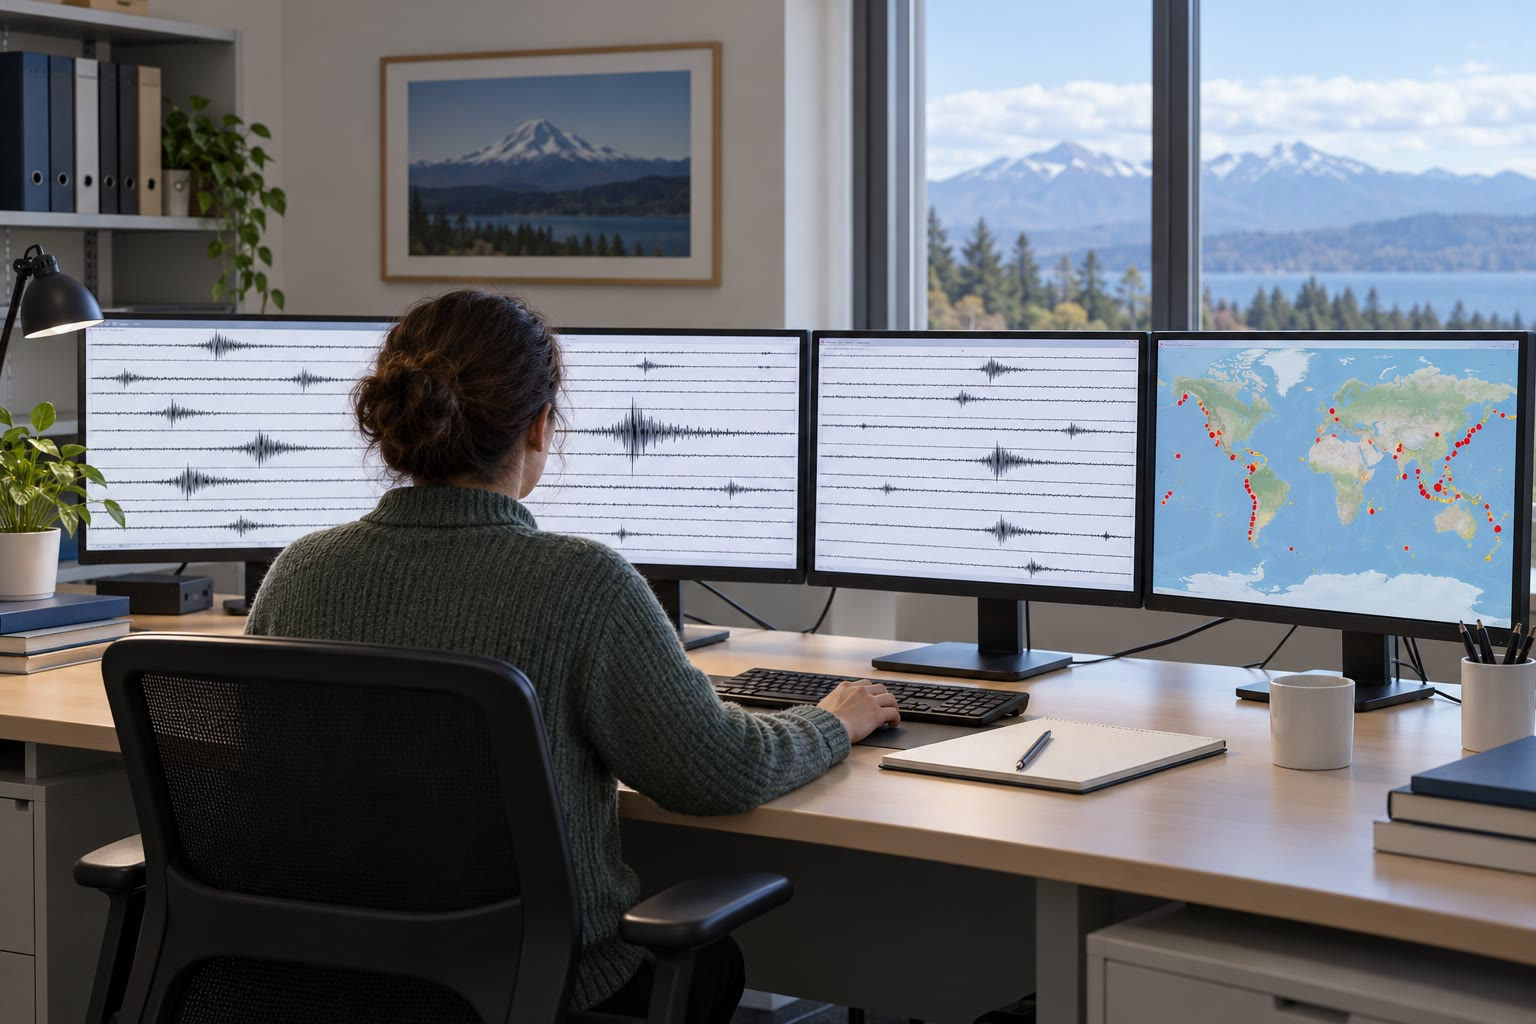
\includegraphics[width=0.66\linewidth]{images/book2/ai/g11-seismology-observatory.jpg}

{\small In a seismology observatory, the records of many stations are shown
side by side, and the earthquakes they locate are plotted on a world map
(AI illustration).}
\end{omfigure}

\section{Refraction and the Moho}\label{sec:g11:seismic-structure:moho}

\subsection{The wave that runs along a boundary}

Inside the Earth the speed of seismic waves changes with depth, mostly
gradually, but in places all at once.

\begin{definition}[Seismic discontinuity]\label{def:g11:seismic-structure:discontinuity}
A \emph{seismic discontinuity}\index{seismic discontinuity} is a surface
inside the Earth across which the speed of seismic waves changes
suddenly --- over a thickness much smaller than the length of the waves.
\end{definition}

At a discontinuity, part of a wave is reflected and part is refracted. Take
a layer of thickness $h$ in which \omterm{def:g11:seismic-structure:body-waves}{P waves} travel at $v_1$, on top of a layer
in which they are faster, $v_2 > v_1$. A ray going down at the angle $i$ from
the vertical is refracted at the angle $r$ given by $\sin r = (v_2/v_1)\sin
i$: it is bent away from the vertical. When $\sin i$ reaches $v_1/v_2$, the
refracted ray runs exactly along the boundary. The angle
\[
  i_c, \qquad \sin i_c = \frac{v_1}{v_2},
\]
is the \emph{critical angle}\index{critical angle}. The wave refracted at the
\omterm{ex:g11:seismic-structure:sp}{critical angle} travels along the top of the faster layer at the speed $v_2$,
and as it goes it sends waves back up into the upper layer, all at the angle
$i_c$: they reach the surface as the \emph{head wave}\index{head wave}.

\begin{omfigure}
\begin{tikzpicture}[x=0.05cm, y=0.05cm, font=\footnotesize, >={Stealth[length=4pt]}]
% geometry from figdata/grade-11/moho_refraction.py: v1 6.2, v2 8.1, h 30 km, ic 49.9 deg
  \fill[omLithGranite!45] (-10,0) rectangle (215,-30);
  \fill[omLithPeridotite!45] (-10,-30) rectangle (215,-48);
  \draw[line width=0.6pt] (-10,0) -- (215,0);
  \draw[line width=0.9pt] (-10,-30) -- (215,-30);
  \node[anchor=west, align=left] at (218,-15) {crust\\$v_1 = \qty{6.2}{km/s}$};
  \node[anchor=west, align=left] at (218,-39) {mantle\\$v_2 = \qty{8.1}{km/s}$};
  \node[anchor=east] at (215,-26) {Moho};
  % source and station
  \fill[omDef] (0,0) circle (1.6);
  \node[anchor=south] at (0,1.5) {earthquake};
  \draw[fill=white] (197,0) -- (203,0) -- (200,5) -- cycle;
  \node[anchor=south] at (200,5) {station};
  % direct wave
  \draw[->, omProp, line width=0.8pt] (2,-2) -- (196,-2);
  \node[anchor=south, text=omProp] at (100,0.3) {direct wave, speed $v_1$};
  % head wave
  \draw[omDef, line width=0.9pt] (0,0) -- (35.7,-30);
  \draw[->, omDef, line width=0.9pt] (35.7,-30) -- (100,-30);
  \draw[omDef, line width=0.9pt] (100,-30) -- (164.3,-30) -- (200,0);
  \node[anchor=north, text=omDef] at (100,-31) {along the Moho at $v_2$};
  \foreach \x in {50,70,90,110,130,150} {
    \draw[->, omDef!60, densely dashed] (\x,-30) -- ++(25.5,21.5);
  }
  % critical angle
  \draw[black!60, densely dotted] (35.7,-30) -- (35.7,-8);
  \draw[black!70] (35.7,-18) arc[start angle=90, end angle=130.05, radius=12];
  \node[anchor=south east] at (33,-16) {$i_c$};
  % thickness and critical distance
  \draw[<->] (-6,0) -- (-6,-30);
  \node[anchor=east] at (-7,-15) {$h$};
\end{tikzpicture}

{\small The direct wave and the \omterm{ex:g11:seismic-structure:sp}{head wave} (to scale: crust \qty{30}{km}
thick). The \omterm{ex:g11:seismic-structure:sp}{head wave} goes down at the \omterm{ex:g11:seismic-structure:sp}{critical angle} $i_c$, runs along the
top of the mantle and comes back up at $i_c$; along its whole path on the
\omterm{def:g11:seismic-structure:moho}{Moho} it sends waves up to the surface (dashed). It reaches no station closer
than $2h\tan i_c$, about \qty{71}{km} here.}
\end{omfigure}

\begin{proposition}[Travel time of the head wave]\label{prop:g11:seismic-structure:head-wave}
For a source at the surface, a station at the distance $x \ge 2h\tan i_c$
receives the \omterm{ex:g11:seismic-structure:sp}{head wave} after
\[
  t(x) = \frac{x}{v_2} + \frac{2h\cos i_c}{v_1}.
\]
Its \omterm{def:g11:seismic-structure:travel-time}{travel-time curve} is a straight line of slope $1/v_2$ which, extended
back, cuts the time axis at the \emph{intercept time}\index{intercept time}
$t_i = 2h\cos i_c/v_1$.
\end{proposition}

\begin{proof}
The ray goes down a slanted leg of length $h/\cos i_c$, which advances
horizontally by $h\tan i_c$; it does the same on the way up. In between it
runs along the boundary for $x - 2h\tan i_c$. The time is
\[
  t = \frac{2h}{v_1\cos i_c} + \frac{x - 2h\tan i_c}{v_2}
    = \frac{x}{v_2} + \frac{2h}{v_1\cos i_c} - \frac{2h\sin i_c}{v_2\cos i_c}.
\]
Since $1/v_2 = \sin i_c/v_1$, the last two terms make
$\frac{2h}{v_1\cos i_c}\,(1 - \sin^2 i_c) = \frac{2h\cos i_c}{v_1}$.
\end{proof}

The direct wave arrives after $x/v_1$: its curve is a line through the
origin, steeper than the head-wave line. Near the source the direct wave comes
first; far away, the \omterm{ex:g11:seismic-structure:sp}{head wave}, which has run most of the way at the higher
speed, overtakes it.

\begin{proposition}[Crossover distance]\label{prop:g11:seismic-structure:crossover}
The \omterm{ex:g11:seismic-structure:sp}{head wave} arrives before the direct wave beyond the \emph{crossover
distance}\index{crossover distance}
\[
  x_c = 2h\sqrt{\frac{v_2 + v_1}{v_2 - v_1}}.
\]
\end{proposition}

\begin{proof}
The two arrive together when $x/v_1 = x/v_2 + 2h\cos i_c/v_1$, that is
$x\,(v_2 - v_1)/(v_1 v_2) = 2h\cos i_c/v_1$, so $x = 2h\cos i_c\,v_2/(v_2 -
v_1)$. Now $\cos i_c = \sqrt{1 - v_1^2/v_2^2} = \sqrt{(v_2 - v_1)(v_2 +
v_1)}/v_2$, hence $x = 2h\sqrt{(v_2 + v_1)(v_2 - v_1)}/(v_2 - v_1) =
2h\sqrt{(v_2 + v_1)/(v_2 - v_1)}$. Beyond it the \omterm{ex:g11:seismic-structure:sp}{head wave}, whose line is
less steep, arrives first.
\end{proof}

\begin{omfigure}
\begin{tikzpicture}
\begin{axis}[omrecord, width=0.78\linewidth, height=5.6cm, xmin=0, xmax=300, ymin=0, ymax=50,
  xtick={0,50,...,300}, xlabel={distance from the epicentre (\unit{km})}, ylabel={travel time (\unit{s})},
  tick label style={font=\small}, label style={font=\small}, clip=false]
% computed in figdata/grade-11/moho_refraction.py (critical_km 71.4, crossover_km 164.6, intercept_s 6.23)
\addplot[omProp, line width=0.9pt] table[x=x, y=tdirect] {figdata/out/grade-11-moho_refraction-model.dat};
\addplot[omDef, line width=0.9pt, restrict x to domain=71:300] table[x=x, y=thead] {figdata/out/grade-11-moho_refraction-model.dat};
\addplot[omDef, densely dashed, restrict x to domain=0:72] table[x=x, y=thead] {figdata/out/grade-11-moho_refraction-model.dat};
\draw[black!50, densely dotted] (axis cs:164.6,0) -- (axis cs:164.6,26.5);
\node[font=\scriptsize, anchor=north] at (axis cs:164.6,0) {$x_c$};
\fill (axis cs:0,6.23) circle (1.5pt);
\draw[black!60] (axis cs:0.8,6.6) -- (axis cs:6,12);
\node[font=\scriptsize, anchor=south west, inner sep=1pt] at (axis cs:5,12) {$t_i = \qty{6.2}{s}$};
\node[font=\small, text=omProp, anchor=south east] at (axis cs:250,41) {direct wave};
\node[font=\small, text=omDef, anchor=north west] at (axis cs:235,33) {head wave};
\end{axis}
\end{tikzpicture}

{\small \omterm{def:g11:seismic-structure:travel-time}{Travel times} of the direct wave and of the \omterm{ex:g11:seismic-structure:sp}{head wave} for the crust
of the previous figure. The head-wave line, extended back (dashed), cuts the
time axis at the \omterm{prop:g11:seismic-structure:head-wave}{intercept time}; beyond the \omterm{prop:g11:seismic-structure:crossover}{crossover distance} $x_c \approx
\qty{165}{km}$ the \omterm{ex:g11:seismic-structure:sp}{head wave} arrives first.}
\end{omfigure}

\subsection{The base of the crust}

\begin{definition}[Moho]\label{def:g11:seismic-structure:moho}
The \emph{Mohorovičić discontinuity}\index{Mohorovičić discontinuity}, or
\emph{Moho}\index{Moho}, is the \omterm{def:g11:seismic-structure:discontinuity}{seismic discontinuity} at the base of the
crust, where the speed of \omterm{def:g11:seismic-structure:body-waves}{P waves} jumps from at most about \qty{7}{km/s}
to about \qty{8}{km/s}, the speed in the uppermost mantle.
\end{definition}
% ledger: kayal:pn-sn, data:prem (6.8 -> 8.11 at 24.4 km)

\begin{history}[Mohorovičić and the two P waves, 1909]
Andrija Mohorovičić (1857--1936) found, on the records of the 1909
earthquake, that beyond a certain distance --- in general between 100 and
\qty{150}{km} --- a weak, faster \omterm{def:g11:seismic-structure:body-waves}{P wave} arrived before the strong \omterm{def:g11:seismic-structure:body-waves}{P wave}.
He explained it as a wave that had travelled through faster rock beneath the
crust. He named the two waves Pg (the direct wave in the crust) and Pn (the
\omterm{ex:g11:seismic-structure:sp}{head wave} along the top of the mantle), did the same for \omterm{def:g11:seismic-structure:body-waves}{S waves}, and
deduced the speeds of both layers and the depth of the boundary between them.
The Pn wave travels at about \qty{8.0}{km/s}, the speed of the uppermost
mantle. His papers of 1910 proved that the crust and the mantle are
different; the boundary carries his name.
\end{history}
% ledger: kayal:pn-sn, srl:mohorovicic

\begin{method}[Depth of the Moho from a travel-time diagram]\label{met:g11:seismic-structure:moho}
\begin{enumerate}
  \item Plot the first arrival times against the distance from the
        epicentre.
  \item Draw the line of the direct wave (through the origin) and the line
        of the \omterm{ex:g11:seismic-structure:sp}{head wave}; their slopes are $1/v_1$ and $1/v_2$.
  \item Extend the head-wave line back to the time axis: it cuts it at the
        \omterm{prop:g11:seismic-structure:head-wave}{intercept time} $t_i$.
  \item With $\sin i_c = v_1/v_2$, the thickness of the crust is
        $h = \dfrac{v_1\,t_i}{2\cos i_c}$.
\end{enumerate}
\end{method}

\begin{example}[A crust \qty{30}{km} thick]\label{ex:g11:seismic-structure:moho}
With $v_1 = \qty{6.2}{km/s}$ and $v_2 = \qty{8.1}{km/s}$, $\sin i_c = 0.765$,
$i_c \approx \ang{49.9}$ and $\cos i_c \approx 0.644$. An \omterm{prop:g11:seismic-structure:head-wave}{intercept time} of
\qty{6.23}{s} gives $h = 6.2 \times 6.23/(2 \times 0.644) \approx
\qty{30}{km}$. The \omterm{ex:g11:seismic-structure:sp}{head wave} first reaches the surface at
$2h\tan i_c \approx \qty{71}{km}$ and overtakes the direct wave beyond
$x_c = 60\sqrt{14.3/1.9} \approx \qty{165}{km}$.
\end{example}
% values computed in figdata/grade-11/moho_refraction.py (ic_deg 49.9, critical_km 71.4, crossover_km 164.6)

Measured in this way all over the world, the \omterm{def:g11:seismic-structure:moho}{Moho} lies only about
\qty{5}{km} below the floor of the oceans. Under the continents it lies about
\qty{41}{km} down on average: about \qty{30}{km} where the crust has been
stretched, more than \qty{45}{km} under mountain belts, and down to about
\qty{100}{km} under the highest ranges. The crust is a thin skin: even
\qty{41}{km} is less than one per cent of the Earth's radius.
% ledger: usgs:crust-thickness, cm95:crust, kayal:discontinuities

\section{The core}

\subsection{Rays that curve}

In the mantle, the speed of seismic waves increases with depth. A ray that
goes down crosses faster and faster rock and, by Snell's law, is bent a
little more away from the vertical at each step: its path curves and turns
back up towards the surface. The deeper a ray turns, the farther from the
earthquake it comes back up. The figure shows such rays, computed with the
speeds of the \omterm{def:g11:seismic-structure:reference-model}{reference Earth model}.

\begin{omfigure}
\begin{tikzpicture}
\begin{axis}[width=0.66\linewidth, height=0.66\linewidth, axis equal image, hide axis,
  xmin=-1.18, xmax=1.18, ymin=-1.18, ymax=1.2, clip=false]
% computed in figdata/grade-11/seismic_rays.py; ledger: data:prem
\fill[omLithPeridotite!25] (axis cs:0,0) circle [radius=1];
\fill[omSea!45] (axis cs:0,0) circle [radius=0.5462];
\fill[omSea!80] (axis cs:0,0) circle [radius=0.1917];
\addplot[black, line width=0.6pt, domain=0:360, samples=181] ({cos(x)}, {sin(x)});
\addplot[black!60, line width=0.4pt, domain=0:360, samples=181] ({0.5462*cos(x)}, {0.5462*sin(x)});
\addplot[black!60, line width=0.4pt, domain=0:360, samples=91] ({0.1917*cos(x)}, {0.1917*sin(x)});
\addplot[omDef, line width=0.6pt] table {figdata/out/grade-11-seismic_rays-praysmantle.dat};
\addplot[omDef!70!black, line width=0.6pt] table {figdata/out/grade-11-seismic_rays-prayscore.dat};
\addplot[omProp, line width=0.6pt] table {figdata/out/grade-11-seismic_rays-srays.dat};
% P shadow zone: 98.5 to 143.8 degrees from the source (right); S beyond 102.7 (left)
\addplot[black!80, line width=3pt, domain=-53.8:-8.5, samples=40] ({1.04*cos(x)}, {1.04*sin(x)});
\addplot[omProp!60, line width=3pt, domain=192.7:270, samples=40] ({1.04*cos(x)}, {1.04*sin(x)});
\fill[omDef] (axis cs:0,1) circle (2pt);
\node[font=\footnotesize, anchor=south] at (axis cs:0,1.04) {earthquake};
\node[font=\footnotesize, anchor=west, align=left] at (axis cs:1.07,-0.42) {no direct P\\(\ang{99}--\ang{144})};
\node[font=\footnotesize, anchor=east, align=right] at (axis cs:-1.07,-0.62) {no direct S\\beyond \ang{103}};
\node[font=\footnotesize, text=omDef, anchor=south west] at (axis cs:0.55,0.8) {P};
\node[font=\footnotesize, text=omProp, anchor=south east] at (axis cs:-0.55,0.8) {S};
\node[font=\scriptsize] at (axis cs:-0.5,-0.62) {mantle};
\node[font=\scriptsize] at (axis cs:-0.3,0.2) {outer core};
\draw[black!70] (axis cs:-0.1,-0.06) -- (axis cs:-0.26,-0.22);
\node[font=\scriptsize, anchor=north east, inner sep=1pt] at (axis cs:-0.24,-0.22) {inner core};
\end{axis}
\end{tikzpicture}

{\small Rays from an earthquake at the top of the Earth, computed with the
speeds of the reference model. Right: P rays that turn in the mantle, out to
about \ang{99}, and P rays that cross the core and come out beyond about
\ang{144}; in between, no P ray arrives directly. Left: S rays, which turn in
the mantle; none crosses the liquid outer core, and no direct \omterm{def:g11:seismic-structure:body-waves}{S wave} reaches
beyond about \ang{103}.}
\end{omfigure}

\subsection{The shadow zone and the liquid outer core}

In 1906, the seismologist Oldham noticed that \omterm{def:g11:seismic-structure:body-waves}{P waves} recorded on the far side
of the Earth from an earthquake arrived late compared with the times
expected, and proposed a central core in which they travel more slowly. In
1912 Gutenberg showed that \omterm{def:g11:seismic-structure:body-waves}{P waves} do not reach a whole band of distances,
between about \ang{105} and \ang{143}, with strong arrivals just beyond
\ang{143}; in 1914 he placed the top of the core \qty{2900}{km} down.
% ledger: kayal:discontinuities, kayal:shadow

\begin{definition}[Shadow zone]\label{def:g11:seismic-structure:shadow-zone}
The \emph{shadow zone}\index{shadow zone} of a seismic wave is the range of
epicentral distances that the wave cannot reach directly from an
earthquake, because the core bends it away or stops it.
\end{definition}

The rays explain it. The P rays that turn just above the core come back up
about \ang{100} from the earthquake. A ray that goes a little steeper
enters the core, where the P speed drops suddenly from \qty{13.7}{km/s} to
about \qty{8.1}{km/s}: by Snell's law it is bent \emph{towards} the vertical,
crosses the core and emerges much farther away, beyond about \ang{144}. No P
ray turning in the mantle and no P ray crossing the core lands in between.
In the reference model the P \omterm{def:g11:seismic-structure:shadow-zone}{shadow zone} runs from \ang{98.5} to
\ang{143.8}, close to Gutenberg's \ang{105}--\ang{143}.
% ledger: kayal:shadow, data:prem (vp_above_cmb 13.72, vp_below_cmb 8.06); computed in
% figdata/grade-11/seismic_rays.py (shadow_start_deg 98.5, shadow_end_pkp_deg 143.8)

\omterm{def:g11:seismic-structure:body-waves}{S waves} tell more. No \omterm{def:g11:seismic-structure:body-waves}{S wave} crosses the outer core: the outer core does not
carry shear waves, so it is liquid. As a result, no \omterm{def:g11:seismic-structure:body-waves}{S wave} arrives directly
beyond about \ang{103} in the reference model --- on the whole far side of
the Earth.
% ledger: kayal:outer-core-liquid; computed in figdata/grade-11/seismic_rays.py (s_direct_max_deg 102.7)

\begin{definition}[Core--mantle boundary; inner-core boundary]\label{def:g11:seismic-structure:core}
The \emph{core--mantle boundary}\index{core--mantle boundary} is the \omterm{def:g11:seismic-structure:discontinuity}{seismic
discontinuity} between the solid mantle and the liquid outer core, at a depth
of \qty{2891}{km}; there the P speed drops from about \qty{13.7}{km/s} to
about \qty{8.1}{km/s}, and \omterm{def:g11:seismic-structure:body-waves}{S waves} stop. The \emph{inner-core
boundary}\index{inner-core boundary}, at a depth of \qty{5150}{km}, separates
the liquid outer core from the solid inner core; there the P speed jumps from
about \qty{10.4}{km/s} to about \qty{11.0}{km/s}.
\end{definition}
% ledger: data:prem, prem:cmb, prem:icb (Book 3 rows); values in figdata/grade-11/prem_profiles.py

The \omterm{def:g11:seismic-structure:shadow-zone}{shadow zone} is not completely silent: weak \omterm{def:g11:seismic-structure:body-waves}{P waves} arrive in it. Inge
Lehmann explained them in 1936 with a solid inner core in which \omterm{def:g11:seismic-structure:body-waves}{P waves}
travel faster (Book 1, grade 6). The rays show how. A P ray that reaches the
inner core is bent away from the vertical where the speed jumps up, as at the
\omterm{def:g11:seismic-structure:moho}{Moho}, and comes back out of the core sooner: in the reference model, rays
through the inner core reach the surface from about \ang{121} on, inside the
\omterm{def:g11:seismic-structure:shadow-zone}{shadow zone} (dotted curve of the travel-time figure).
% ledger: nbi:lehmann-1936 (Book 1 row), kayal:lehmann; computed in
% figdata/grade-11/seismic_rays.py (pkikp_min_deg 121.4)

\section{A reference Earth model}\label{sec:g11:seismic-structure:model}

Put together, millions of \omterm{def:g11:seismic-structure:travel-time}{travel times} give the speed of P and \omterm{def:g11:seismic-structure:body-waves}{S waves} at
every depth. Their speeds depend on the rock and on its density, and the
total mass of the Earth fixes its average density; together they give the
density at every depth too.
% ledger: data:prem, prem:constraints (Book 3 row)

\begin{definition}[Reference Earth model]\label{def:g11:seismic-structure:reference-model}
A \emph{reference Earth model}\index{reference Earth model} is a table of the
speed of \omterm{def:g11:seismic-structure:body-waves}{P waves}, the speed of \omterm{def:g11:seismic-structure:body-waves}{S waves} and the density against depth, the
same in every direction, chosen to agree with the observed \omterm{def:g11:seismic-structure:travel-time}{travel times} of
seismic waves and with the mass of the Earth.
\end{definition}

The most used is the Preliminary Reference Earth Model (PREM), published by
A.~M.~Dziewonski and D.~L.~Anderson in 1981. The rays and \omterm{def:g11:seismic-structure:travel-time}{travel times} of this
chapter were computed with it: the P \omterm{def:g11:seismic-structure:travel-time}{travel time} at \ang{60}, for instance,
comes out at \qty{607}{s}, against \qty{608}{s} observed.
% ledger: data:prem, auspass:surftim; computed in figdata/grade-11/seismic_rays.py (p_60_s 607.2)

\begin{omfigure}
\begin{tikzpicture}
\begin{axis}[omrecord, width=0.86\linewidth, height=6.2cm, xmin=0, xmax=6371, ymin=0, ymax=14.5,
  xtick={0,1000,...,6000}, ytick={0,2,...,14}, scaled x ticks=false,
  xticklabel style={/pgf/number format/1000 sep={\,}},
  xlabel={depth (\unit{km})}, ylabel={speed (\unit{km/s}) or density (\unit{g/cm^3})},
  tick label style={font=\small}, label style={font=\small}, clip=false]
% computed in figdata/grade-11/prem_profiles.py; ledger: data:prem
\addplot[omDef, line width=0.9pt] table[x=depth, y=vp] {figdata/out/grade-11-prem_profiles-profile.dat};
\addplot[omProp, line width=0.9pt] table[x=depth, y=vs] {figdata/out/grade-11-prem_profiles-profile.dat};
\addplot[black, line width=0.9pt, densely dashed] table[x=depth, y=rho] {figdata/out/grade-11-prem_profiles-profile.dat};
\foreach \d in {670,2891,5149.5} {\edef\temp{\noexpand\draw[black!40, densely dotted] (axis cs:\d,0) -- (axis cs:\d,14.5);}\temp}
\node[font=\scriptsize, anchor=south, align=center] at (axis cs:2891,14.5) {core--mantle\\boundary};
\node[font=\scriptsize, anchor=south, align=center] at (axis cs:5149.5,14.5) {inner-core\\boundary};
\node[font=\scriptsize, anchor=south] at (axis cs:670,14.5) {\qty{670}{km}};
\node[font=\small, text=omDef, anchor=south] at (axis cs:1800,12.4) {P speed};
\node[font=\small, text=omProp, anchor=south] at (axis cs:1800,7.0) {S speed};
\node[font=\small, anchor=north] at (axis cs:1800,4.5) {density};
\node[font=\scriptsize, align=center] at (axis cs:4000,1.9) {no S waves:\\liquid};
\end{axis}
\end{tikzpicture}

{\small The speeds of P and \omterm{def:g11:seismic-structure:body-waves}{S waves} and the density against depth in the
Preliminary Reference Earth Model (Dziewonski and Anderson, 1981). The
dotted lines mark the main discontinuities below the \omterm{def:g11:seismic-structure:moho}{Moho}, which is too
shallow to show at this scale.}
\end{omfigure}

Reading the model from the top:
\begin{itemize}
  \item the crust, with P speeds of 5.8 to \qty{6.8}{km/s}, ends at the \omterm{def:g11:seismic-structure:moho}{Moho}
        (\qty{24.4}{km} in this average model);
  \item in the mantle, the speeds rise with depth, with smaller sudden
        steps, the largest near \qty{400}{km} and \qty{670}{km};
  \item at \qty{2891}{km}, the S speed falls to zero and the P speed drops
        by more than \qty{5}{km/s}: the liquid outer core;
  \item at \qty{5150}{km}, \omterm{def:g11:seismic-structure:body-waves}{S waves} exist again: the solid inner core,
        \qty{1220}{km} in radius.
\end{itemize}
% ledger: data:prem (discontinuities in figdata/grade-11/prem_profiles.py)

The density rises from \qty{2.6}{g/cm^3} in the crust to
\qty{5.6}{g/cm^3} at the base of the mantle, then jumps to
\qty{9.9}{g/cm^3} at the top of the core and reaches \qty{13.1}{g/cm^3} at
the centre. The mean density of the whole model is \qty{5.5}{g/cm^3}, twice
that of the rocks of the crust: the deep interior, and the core above all, is
made of much denser material than the surface. The core holds about one
third of the Earth's mass.
% ledger: data:prem, prem:cmb, prem:centre (Book 3 rows); computed in
% figdata/grade-11/prem_profiles.py (mean_density 5.52; core mass fraction 0.32)

\section{Exercises}

\begin{exercise}[$\star$]\label{exo:g11:seismic-structure:1}
Give two differences between \omterm{def:g11:seismic-structure:body-waves}{P waves} and \omterm{def:g11:seismic-structure:body-waves}{S waves}. Which one is recorded first
by a seismometer, and why?
\end{exercise}

\begin{exercise}[$\star$]\label{exo:g11:seismic-structure:2}
A station lies \ang{40} from an epicentre. How far is it, measured along the
surface? How many degrees away is a station \qty{8900}{km} from an
epicentre?
\end{exercise}

\begin{exercise}[$\star$]\label{exo:g11:seismic-structure:3}
The observed \omterm{def:g11:seismic-structure:travel-time}{travel times} at \ang{40} are \qty{456}{s} for P and
\qty{822}{s} for S. Convert them to minutes and seconds, and give the S--P
delay.
\end{exercise}

\begin{exercise}[$\star$]\label{exo:g11:seismic-structure:4}
A crust in which \omterm{def:g11:seismic-structure:body-waves}{P waves} travel at \qty{6.0}{km/s} lies on a mantle where
they travel at \qty{8.0}{km/s}. Compute the \omterm{ex:g11:seismic-structure:sp}{critical angle}.
\end{exercise}

\begin{exercise}[$\star$]\label{exo:g11:seismic-structure:5}
In the reference model the \omterm{def:g11:seismic-structure:core}{core--mantle boundary} lies \qty{2891}{km} deep and
the \omterm{def:g11:seismic-structure:core}{inner-core boundary} \qty{5150}{km} deep; the Earth's radius is
\qty{6371}{km}. Compute the thickness of the outer core, the radius of the
core, and the core's radius as a fraction of the Earth's radius.
\end{exercise}

\begin{exercise}[$\star\star$]\label{exo:g11:seismic-structure:6}
Observed S--P delays are \qty{224}{s} at \ang{20}, \qty{298}{s} at
\ang{30}, \qty{366}{s} at \ang{40}, \qty{431}{s} at \ang{50} and
\qty{493}{s} at \ang{60}. A station records an \omterm{def:g11:seismic-structure:body-waves}{S wave} 6~minutes 6~seconds
after the \omterm{def:g11:seismic-structure:body-waves}{P wave}. How far is the earthquake, in degrees and in kilometres?
Why can a single station not tell where the earthquake is?
\end{exercise}

\begin{exercise}[$\star\star$]\label{exo:g11:seismic-structure:7}
With the speeds of \cref{exo:g11:seismic-structure:4} and a crust
\qty{35}{km} thick, compute the \omterm{def:g11:seismic-structure:travel-time}{travel times} of the direct wave and of the
\omterm{ex:g11:seismic-structure:sp}{head wave} at a station \qty{200}{km} from the epicentre. Which arrives first?
\end{exercise}

\begin{exercise}[$\star\star$]\label{exo:g11:seismic-structure:8}
For the crust of \cref{exo:g11:seismic-structure:7}, compute the critical
distance $2h\tan i_c$ and the \omterm{prop:g11:seismic-structure:crossover}{crossover distance}. Check that the answer to
\cref{exo:g11:seismic-structure:7} agrees.
\end{exercise}

\begin{exercise}[$\star\star$]\label{exo:g11:seismic-structure:9}
Under an ocean, a crust \qty{6}{km} thick, in which \omterm{def:g11:seismic-structure:body-waves}{P waves} travel at
\qty{6.5}{km/s}, lies on a mantle at \qty{8.0}{km/s}. Compute the \omterm{ex:g11:seismic-structure:sp}{critical
angle}, the \omterm{prop:g11:seismic-structure:head-wave}{intercept time} and the \omterm{prop:g11:seismic-structure:crossover}{crossover distance}. Why must the stations be
much closer together to find the \omterm{def:g11:seismic-structure:moho}{Moho} beneath an ocean than beneath a
continent?
\end{exercise}

\begin{exercise}[$\star\star$]\label{exo:g11:seismic-structure:10}
A P ray in the lowest mantle, where it travels at \qty{13.7}{km/s}, meets the
\omterm{def:g11:seismic-structure:core}{core--mantle boundary} at \ang{30} from the perpendicular. Below the boundary
the P speed is \qty{8.06}{km/s}. Compute the angle of the refracted ray. Is the
ray bent towards the perpendicular or away from it? Use this to explain why P
rays that enter the core emerge far from the earthquake.
\end{exercise}

\begin{exercise}[$\star\star$]\label{exo:g11:seismic-structure:11}
In the reference model, a \omterm{def:g11:seismic-structure:body-waves}{P wave} going straight down through the centre takes
\qty{1210}{s} to reach the opposite point of the Earth. How long would it take
if it travelled the whole diameter (\qty{12742}{km}) at \qty{13.7}{km/s}, the
P speed at the base of the mantle? What did Oldham conclude from such delays?
\end{exercise}

\begin{exercise}[$\star\star\star$]\label{exo:g11:seismic-structure:12}
(1) From \cref{prop:g11:seismic-structure:head-wave}, show that the thickness
of the crust is
\[
  h = \frac{t_i\,v_1 v_2}{2\sqrt{v_2^2 - v_1^2}}.
\]
(2) Apply it to $t_i = \qty{6.23}{s}$, $v_1 = \qty{6.2}{km/s}$ and
$v_2 = \qty{8.1}{km/s}$.
\end{exercise}

\begin{exercise}[$\star\star\star$]\label{exo:g11:seismic-structure:13}
The mean density of the Earth is \qty{5.52}{g/cm^3}. Treat the Earth as a
core of radius \qty{3480}{km} and uniform density $\rho_c$, inside a mantle
and crust of uniform density \qty{4.45}{g/cm^3} (the mean of the reference
model). (1) What fraction of the Earth's volume is the core? (2) Compute
$\rho_c$. (3) Compare with the density at the top of the core in the
reference model, \qty{9.9}{g/cm^3}, and with the density of the crust.
\end{exercise}

\begin{exercise}[$\star\star\star$]\label{exo:g11:seismic-structure:14}
Gutenberg's P \omterm{def:g11:seismic-structure:shadow-zone}{shadow zone} extends from \ang{105} to \ang{143}. (1) Give its
limits in kilometres along the surface. (2) On a sphere, the area between the
angular distances $a$ and $b$ from a point is the fraction $(\cos a - \cos
b)/2$ of the whole surface. What fraction of the Earth's surface receives no
direct \omterm{def:g11:seismic-structure:body-waves}{P wave} from a given earthquake? (3) Why does every earthquake have its
own \omterm{def:g11:seismic-structure:shadow-zone}{shadow zone}?
\end{exercise}

\begin{exercise}[$\star\star\star$]\label{exo:g11:seismic-structure:15}
Under a high mountain range, a refraction survey finds $v_1 =
\qty{6.3}{km/s}$, $v_2 = \qty{8.1}{km/s}$ and an \omterm{prop:g11:seismic-structure:head-wave}{intercept time} of
\qty{9.5}{s}. (1) Compute the thickness of the crust there. (2) What
\omterm{prop:g11:seismic-structure:head-wave}{intercept time} would a crust \qty{30}{km} thick with the same speeds give?
(3) Compare with the average thickness of the continental crust.
\end{exercise}

\section{Problem: Finding the Moho}

\begin{problem}[{Weekend problem --- the depth of the crust from fifteen stations}]
\label{pb:g11:seismic-structure:1}
% readings computed in figdata/grade-11/moho_refraction.py (part stations; invented region,
% v1 6.2, v2 8.1, h 30 km, reading errors of up to 0.1 s); ledger: kayal:pn-sn, usgs:crust-thickness
A small earthquake occurs at a very shallow depth beneath a continent.
Fifteen stations set out on a straight line from the epicentre record the
arrival times of the first \omterm{def:g11:seismic-structure:body-waves}{P wave} and, where they can be read, of a second
one. The readings below are invented, but computed as a real survey would
find them, to the nearest tenth of a second. Pg is the wave that travels
through the crust, Pn the one that has run along the top of the mantle.

\begin{center}
\small
\begin{tabular}{|c|c|c||c|c|c|}
\hline
distance (\unit{km}) & Pg (\unit{s}) & Pn (\unit{s}) & distance (\unit{km}) & Pg (\unit{s}) & Pn (\unit{s}) \\ \hline
20 & 3.3 & --- & 180 & 29.0 & 28.5 \\ \hline
40 & 6.5 & --- & 200 & 32.3 & 30.9 \\ \hline
60 & 9.7 & --- & 220 & --- & 33.3 \\ \hline
80 & 12.8 & 16.2 & 240 & --- & 35.8 \\ \hline
100 & 16.1 & 18.6 & 260 & --- & 38.3 \\ \hline
120 & 19.3 & 21.1 & 280 & --- & 40.8 \\ \hline
140 & 22.6 & 23.6 & 300 & --- & 43.2 \\ \hline
160 & 25.8 & 26.0 & & & \\ \hline
\end{tabular}
\end{center}

\medskip
\noindent\textbf{Part I --- The direct wave.}
\begin{enumerate}
  \item On graph paper, plot the Pg and Pn times against distance (\qty{1}{cm}
        for \qty{20}{km} and for \qty{5}{s}). How do the Pg points lie?
  \item Why does the Pg line pass close to the origin?
  \item Using the stations at 20 and \qty{200}{km}, compute the slope of the
        Pg line in seconds per kilometre.
  \item Deduce the speed $v_1$ of \omterm{def:g11:seismic-structure:body-waves}{P waves} in the crust.
  \item If the crust continued, when would the Pg wave reach the station at
        \qty{300}{km}?
\end{enumerate}

\medskip
\noindent\textbf{Part II --- The refracted wave.}
\begin{enumerate}[resume]
  \item Using the stations at 100 and \qty{300}{km}, compute the slope of the
        Pn line and the speed $v_2$ of \omterm{def:g11:seismic-structure:body-waves}{P waves} beneath the crust.
  \item Compare $v_2$ with the speed of the Pn wave that Mohorovičić measured,
        about \qty{8.0}{km/s}. What rock lies beneath the crust?
  \item Compute the \omterm{ex:g11:seismic-structure:sp}{critical angle} $i_c$.
  \item No station closer than \qty{80}{km} records a Pn wave. Using
        \cref{prop:g11:seismic-structure:head-wave}, explain why there is a
        smallest distance at which the \omterm{ex:g11:seismic-structure:sp}{head wave} can be recorded.
  \item Between 80 and \qty{160}{km}, Pn arrives after Pg. Why is it still
        recorded?
\end{enumerate}

\medskip
\noindent\textbf{Part III --- The crossover.}
\begin{enumerate}[resume]
  \item From the table, between which two stations does the first wave to
        arrive change from Pg to Pn?
  \item Write the equations of the two lines, using the points at
        \qty{20}{km} (Pg) and \qty{100}{km} (Pn).
  \item Compute the distance at which the two lines cross.
  \item Beyond \qty{200}{km} no station records Pg as a separate wave. Which
        wave does a station at \qty{250}{km} record first, and when?
\end{enumerate}

\medskip
\noindent\textbf{Part IV --- The depth of the Moho.}
\begin{enumerate}[resume]
  \item Extend the Pn line back to the time axis: what is the \omterm{prop:g11:seismic-structure:head-wave}{intercept time}
        $t_i$?
  \item Compute $\cos i_c$, and the thickness $h$ of the crust by
        \cref{met:g11:seismic-structure:moho}.
  \item Check: with this $h$, compute the \omterm{prop:g11:seismic-structure:crossover}{crossover distance} with
        \cref{prop:g11:seismic-structure:crossover} and compare with
        question~13.
  \item Check again: compute the critical distance $2h\tan i_c$ and compare
        with the nearest station that records Pn.
  \item The seismologists give $h$ to the nearest few kilometres only. Why
        is a finer value not justified?
  \item Conclude: at what depth does the \omterm{def:g11:seismic-structure:moho}{Moho} lie beneath this region? Is the
        crust here thin or thick for a continent?
\end{enumerate}
\end{problem}
